\subsection{Движение по орбите}

\term{Закон сохранения момента импульса}:  векторная сумма моментов 
импульса замкнутой системы тел относительно выбранной оси остается 
постоянной, если суммарный момент $\vec{M}$ внешних сил, действующих на систему, равен нулю. Иначе,
\begin{equation}
\vec{L} \equiv \sum\limits_{i=1}^{n} \left[ \vec{r}_i \times m_i \vec{v}_i \right] = \const.
\end{equation}

\change{Докажем это, доказав равенство нулю производной по времени:
\begin{multline*}
	\frac{d\vec{L}}{dt} =  \sum\limits_{i=1}^n \frac{[d\vec{r}_i \times \vec{p}_i]}{dt} \overset{m_i=\const}{=} \sum\limits_{i=1}^n \left[\frac{d\vec{r}_i}{dt} \times m_i\vec{v}_i \right] + \sum\limits_{i=1}^n \left[\vec{r}_i \times m_i \frac{d\vec{v}_i}{dt} \right] = \\ 
	= \sum\limits_{i=1}^n \underbrace{\left[\vec{v}_i \times m_i\vec{v}_i \right]}_{=\vec{0}} + \sum\limits_{i=1}^n \left[\vec{r}_i \times m_i \vec{a}_i \right] = \\
	= \sum\limits_{i=1}^n \left[ \vec{r}_i \times m_i \sum\limits_{j = 1 }^n \frac{G m_j}{|\vec{r}_j - \vec{r}_i|^3} (\vec{r}_j - \vec{r}_i) \right] = \\
	= \sum\limits_{i,j=1}^n \frac{G m_i m_j}{|\vec{r}_j - \vec{r}_i|^3} \big[\vec{r}_i \times (\vec{r}_j - \vec{r}_i) \big] = \sum\limits_{i,j=1}^n \frac{G m_i m_j}{|\vec{r}_j - \vec{r}_i|^3} [\vec{r}_i \times \vec{r}_j] \equiv \sum\limits_{i,j=1}^n \vec{x}_{ij}.
\end{multline*}
Можно заметить, что $\vec{x}_{ij} = -\vec{x}_{ji}$, так как
\begin{equation*}
	\vec{x}_{ij} \equiv \frac{G m_i m_j}{|\vec{r}_j - \vec{r}_i|^3} [\vec{r}_i \times \vec{r}_j] = - \frac{G m_j m_i}{|\vec{r}_i - \vec{r}_j|^3} [\vec{r}_j \times \vec{r}_i] \equiv \vec{x}_{ji}.
\end{equation*}
Отсюда сразу следует равенство нулю производной по времени полного момента импульса, что заканчивает доказательство его сохранения.
}

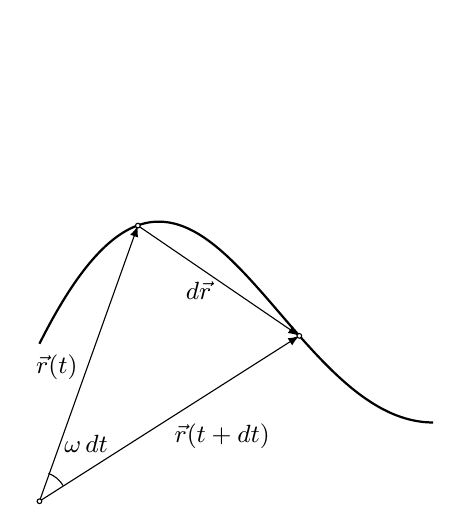
\begin{tikzpicture}
	\small

%	\foreach \x in {0, .1,...,5} {
%		\draw [line width=.1pt] (\x, -3) -- (\x, 3);
%	};
%	
%	\foreach \y in {-3, -2.9,...,3} {
%		\draw [line width=.1pt] (0, \y) -- (5, \y);
%	};

  \draw [thick] (0, 0) .. controls (2, 4) and (3, -1) .. (5, -1);
  \draw [-latex] (0, -2) -- (1.25, 1.5);
  \draw [-latex] (0, -2) -- (3.3, .1);
  \draw [-latex] (1.25, 1.5) -- (3.3, .1);
%  \draw [dashes, -latex] (1.25, 1.5) -- (4.55, 3.6);
%  \draw [dashes, -latex]  (3.3, .1) -- (4.55, 3.6);
%  \draw [-latex] (1.25, 1.5) -- (3.3, .1);
  
  \draw (.3, -1.8) arc(31:70:0.36);
  
  \draw (.6, -.3) node [anchor = east] {$\vec{r}(t)$};
  \draw (1.6, -.9) node [anchor = north west] {$\vec{r}(t + dt)$};
  \draw (2.3, 0.9) node [anchor = north east] {$d\vec{r}$};
  \draw (0.2, -1.5) node [anchor = south west] {$\boldsymbol{\omega} \,dt$};
  
  \draw[fill=white] (1.25, 1.5) circle (0.03);
  \draw[fill=white] (3.3, .1) circle (0.03);
  \draw[fill=white] (0, -2) circle (0.03);  

\end{tikzpicture}

\change{Рассмотрим такую физическую величину, как \term{секториальная скорость}~--- это векторная величина, описывающая ориентированную площадь, заметаемую радиус вектором тела за единицу времени. Пусть в момент времени $t$ тело находилось в точке $\vec{r}(t)$, а через промежуток времени $dt$~--- в точке $\vec{r}(t + dt)$. Обозначим перемещение тела за этот промежуток времени как $d\vec{r}$. Его можно выразить через скорость тела в момент времени $t$, считая ее постоянной на промежутке от $t$ до $t + dt$: $d\vec{r} = \vec{v} \, dt$. Площадь, которую заметает радиус-вектор тело $\vec{r}(t)$ равна половине параллелограмма, построенного на векторах $\vec{r}(t)$ и $d\vec{r}$. Поэтому можно записать
\begin{equation*}
	\vec{s} = \frac{1}{2} [\vec{r} \times \vec{v} dt],
\end{equation*}
	следовательно секториальная скорость равна
\begin{equation*}
	\boldsymbol{\sigma} = \frac{d \vec{s}}{dt} = \frac{1}{2} [\vec{r} \times \vec{v}] = \frac{\vec{l}}{2} = \frac{\vec{L}}{2m},
\end{equation*}
где $\vec{l}$~--- удельный момент импульса (на единицу массы). Полученное выражение доказывает \imp{второй закон Кеплера}. 
}

\change{С другой стороны, перемещение $d\vec{r}$ можно выразить через угловую скорость $\boldsymbol{\omega}$, как $d \vec{r} = [\vec{r} \times \boldsymbol{\omega}\,dt]$. Тогда
\begin{equation*}
	\boldsymbol{\sigma} = \frac{1}{2} \big[ \vec{r} \times [\vec{r} \times \boldsymbol{\omega} ]\big] = \vec{r} \underbrace{(\vec{r}, \boldsymbol{\omega})}_0 - \boldsymbol{\omega} ( \vec{r}, \vec{r} ) = r^2 \boldsymbol{\omega}.
\end{equation*}
Получим \imp{третий закон Кеплера}, заметив, что модуль секториальной скорости можно записать, как
\begin{gather*}
	\sigma = \frac{S_\text{эл}}{T} = \frac{\pi a b}{T} = \frac{L}{2m},\\
	\frac{\pi a^2 \sqrt{1 - e^2}}{T} = \frac{m \sqrt{\dfrac{GM}{a} \cdot \dfrac{1 + e}{1 - e}} \cdot a(1-e)}{2m},\\
	\frac{4\pi^2 a^4 (1 - e^2)}{T^2} =a^2(1-e)^2 \cdot \frac{GM}{a} \cdot \frac{1 + e}{1-e}
\end{gather*}
\begin{equation}
	\frac{T^2}{a^3} = \frac{4\pi^2}{GM}.чч
\end{equation}
}

\change{Получим еще одно важное соотношение~--- \term{интеграл энергии}~--- формулу для скорости тела на орбите с большой полуосью $a$ в точке, удалённой на расстояние~$r$ от центрального тела с массой $M$. Для этого рассмотрим  сначала точку перицентра ($q$, <<п>>) и апоцентра ($Q$, <<a>>) данной орбиты, запишем для них закон сохранения энергии и закон сохранения момента импульса:
\begin{gather*}
	-\frac{GMm}{q} + \frac{m v^2_\text{п}}{2} = -\frac{GMm}{Q} + \frac{m v^2_\text{а}}{2},\\
	mv_\text{п}q = mv_\text{a}Q.
\end{gather*}
Из ЗСМИ и выражений для перицентрического $q$ и апоцентрического $Q$ расстояний через большую полуось $a$ и эксцентриситет $e$ имеем:
\begin{equation*}
	\frac{v_\text{а}}{v_\text{п}} = \frac{1 - e}{1 + e}.
	\end{equation*}сИспользую это соотношения, преобразуем ЗСЭ:
\begin{gather}
	\frac{v_\text{п}^2}{2} \left( 1 - \frac{(1 -e)^2}{(1 + e)^2} \right) = GM \left( \frac{1}{a(1-e)} - \frac{1}{a(1+e)} \right),\\
	\frac{v_\text{п}^2}{2} \cdot \frac{ 1 + 2e + e^2 - 1 + 2e - e^2}{(1+e)^2} = \frac{GM}{a} \cdot \frac{1 + e - 1 +  e}{(1+e)(1-e)},\\
	v_\text{п} = \sqrt{\frac{GM}{a}}\sqrt{\frac{1+e}{1-e}}, \quad \quad v_\text{a} = \sqrt{\frac{GM}{a}}\sqrt{\frac{1-e}{1+e}}.
\end{gather}
Запишем теперь ЗСЭ для перицентра и произвольной точки орбиты на расстоянии $r$:
\begin{gather*}
	-\frac{GMm}{q} + \frac{m v^2_\text{п}}{2} = -\frac{GMm}{r} + \frac{m v^2}{2},\\
	-\frac{GMm}{q} + \frac{GMm}{2a} \cdot \frac{1+e}{1-e} = -\frac{GMm}{r} + \frac{m v^2}{2},\\
	v^2 = GM \left( \frac{2}{r} - \frac{2}{a(1 - e)} + \frac{1+e}{a (1-e) }\right) = GM \left( \frac{2}{r} - \frac{1}{a} \right),
\end{gather*}
\begin{equation}
v = \sqrt{ GM \left( \frac{2}{r} - \frac{1}{a} \right)}.
\label{eq:int-energy}
\end{equation}
Полученное выражение и называется интегралом энергии. Согласно \eqref{eq:int-energy} и \eqref{eq:ellipse-pol-eq} для скорости тела в произвольной точке орбиты также справедливо выражение
\begin{equation}
v = \sqrt{\frac{GM}{p}\cdot(1 + 2 e \cos \nu + e^2)},
\end{equation}
где $\nu$~--- истинная аномалия, а $p$~--- фокальный параметр.
}
